\section{Phương pháp Phân vùng Bản đồ & Biểu diễn Ngữ nghĩa}
\label{sec:perception}

Một trong những đóng góp trọng tâm của đề tài là giải pháp tự động chuyển đổi bản đồ hình học dạng lưới tĩnh (\textit{Occupancy Grid Map}) thành bản đồ ngữ nghĩa không gian (\textit{Semantic Map}) thông qua lý thuyết xử lý ảnh hình thái học và giải thuật phân vùng Watershed có kiểm soát (\textit{Marker-Controlled Watershed Segmentation}).

\subsection{Tiền Xử lý Bản đồ Lưới Chiếm chỗ (Occupancy Grid)}

Bản đồ môi trường thực nghiệm được tạo bởi gói SLAM/Gazebo với kích thước thực tế $14.0\,\text{m} \times 11.0\,\text{m}$, độ phân giải $\Delta = 0.05\,\text{m/pixel}$, tương ứng với lưới ma trận pixel kích thước $W = 280$, $H = 220$. Tọa độ gốc đặt tại $(\text{origin}_x, \text{origin}_y) = (-7.0, -5.5)\,\text{m}$.

Mỗi ô lưới có giá trị độ tin cậy chiếm chỗ $M(u, v) \in [0, 100]$ hoặc $-1$ (chưa khám phá). Để phục vụ xử lý hình ảnh, bản đồ được nhị phân hóa sang ảnh không gian tự do $B(u, v)$ theo biểu thức:
\begin{equation}
B(u, v) = \begin{cases}
255, & \text{nếu } M(u, v) = 0 \text{ (Không gian tự do -- Free Space)}, \\
0, & \text{nếu } M(u, v) \ge 50 \text{ hoặc } M(u, v) = -1 \text{ (Tường, Vật cản)}.
\end{cases}
\end{equation}

Nhằm triệt tiêu nhiễu pixel lẻ dọc theo các vách tường mô phỏng, phép toán mở hình thái học (\textit{Morphological Opening}) với phần tử cấu trúc chữ thập $3 \times 3$ ($\mathcal{K}_3$) được áp dụng:
\begin{equation}
B_{\text{clean}} = (B \ominus \mathcal{K}_3) \oplus \mathcal{K}_3
\end{equation}
trong đó $\ominus$ biểu diễn phép co (\textit{Erosion}) và $\oplus$ biểu diễn phép giãn (\textit{Dilation}).

\subsection{Biến đổi Khoảng cách Euclidean (Distance Transform)}

Bản chất của các phòng học và hành lang trong khuôn viên là các vùng mở rộng được ngăn cách bởi các lối đi hẹp (cửa ra vào). Do đó, hàm biến đổi khoảng cách Euclidean đóng vai trò chủ đạo trong việc xác định độ sâu của không gian tự do so với vật cản gần nhất:
\begin{equation}
D(p) = \min_{q \in \mathcal{O}} \|p - q\|_2 = \min_{q \in \mathcal{O}} \sqrt{(u_p - u_q)^2 + (v_p - v_q)^2}
\end{equation}
với $\mathcal{O} = \{(u, v) \mid B_{\text{clean}}(u, v) = 0\}$ là tập hợp các điểm chướng ngại vật và bờ tường.

Trên ma trận khoảng cách $D$, tâm của các căn phòng lớn (nơi cách xa tường nhất) sẽ có giá trị cực đại địa phương (\textit{local maxima}), trong khi các ngưỡng cửa hẹp có khoảng cách nhỏ hơn rất nhiều do gần các mép tường hai bên.

\begin{figure}[H]
\centering
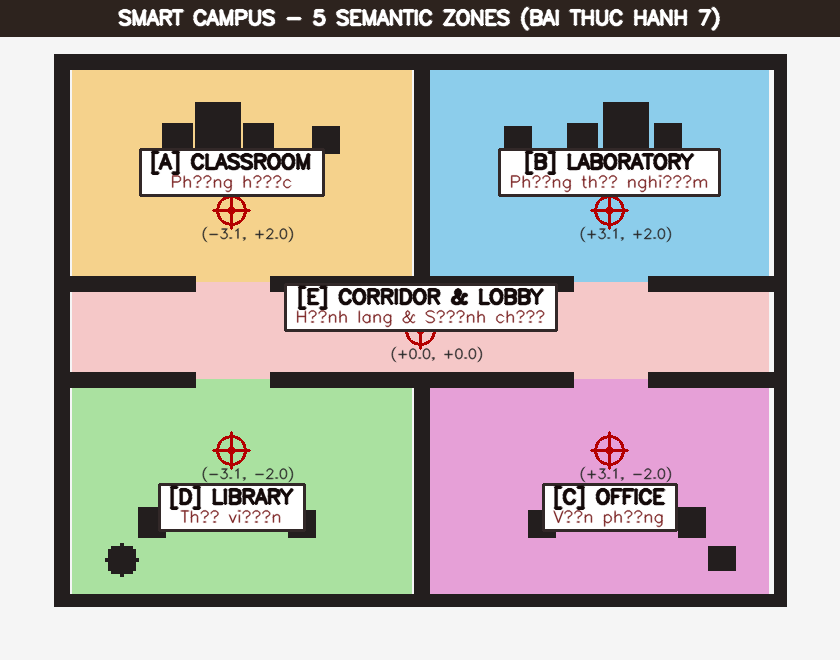
\includegraphics[width=0.88\textwidth]{figures/segmented_map.png}
\caption{Kết quả phân vùng bản đồ tự động bằng giải thuật Marker-controlled Watershed (5 khu vực A, B, C, D, E kèm nhãn nhận diện song ngữ).}
\label{fig:segmented_map}
\end{figure}

\subsection{Trích xuất Hạt giống & Giải thuật Watershed có Kiểm soát}

Để ngăn ngừa hiện tượng phân vùng quá mức (\textit{over-segmentation}) vốn là nhược điểm cố hữu của thuật toán Watershed truyền thống, hệ thống triển khai phương pháp trích xuất hạt giống mầm (\textit{Seed Markers Extraction}) dựa trên ngưỡng động:
\begin{equation}
S = \left\{ (u, v) \mid D(u, v) \ge \tau \cdot \max_{(x, y)} D(x, y) \right\}
\end{equation}
với hệ số ngưỡng được tối ưu hóa $\tau = 0.50$. 

Tập hợp $S$ bao gồm các cụm pixel nằm sâu bên trong lõi mỗi phòng. Bằng thuật toán gán nhãn thành phần liên thông (\textit{Connected Components Labeling}), ta thu được $K$ vùng hạt giống riêng biệt:
\begin{equation}
\mathcal{M} = \bigcup_{k=1}^K \Omega_k, \quad \Omega_i \cap \Omega_j = \emptyset \quad (\forall i \ne j)
\end{equation}

Xem mặt phẳng khoảng cách nghịch đảo $-D(u, v)$ như một bề mặt địa hình 3D với các "thung lũng" tại các hạt giống $\Omega_k$. Thuật toán Watershed tiến hành làm ngập nước địa hình từ các mầm này. Khi các dòng nước từ hai phòng khác nhau gặp nhau tại các khe cửa hẹp (yên ngựa địa hình), một đường đập ngăn (\textit{Watershed dam}) được dựng lên, hình thành ranh giới phân vùng sắc nét giữa các phòng chức năng và trục hành lang.

\subsection{Trích xuất Thuộc tính Hình học & Sinh Điểm Đích (Waypoint Generation)}

Từ ma trận nhãn phân vùng $L(u, v) \in \{1, \dots, K\}$, hệ thống trích xuất các thông số hình học và chuyển đổi sang hệ tọa độ thực thế giới thực $(x, y)_{\text{world}}$:

\begin{enumerate}
    \item \textbf{Tâm hình học (Centroid):}
    \begin{equation}
    \bar{u}_k = \frac{1}{N_k} \sum_{(u, v) \in \text{Zone}_k} u, \quad \bar{v}_k = \frac{1}{N_k} \sum_{(u, v) \in \text{Zone}_k} v
    \end{equation}
    \begin{equation}
    x_{\text{world}} = \text{origin}_x + \bar{u}_k \cdot \Delta, \quad y_{\text{world}} = \text{origin}_y + (H - 1 - \bar{v}_k) \cdot \Delta
    \end{equation}
    
    \item \textbf{Đường bao chữ nhật & Đa giác bao lồi (Bounds & Convex Hull):}
    Xác định phạm vi giới hạn $[x_{\min}, x_{\max}, y_{\min}, y_{\max}]$ phục vụ việc kiểm tra vị trí hiện tại của robot (\textit{Point-in-Polygon Check}) một cách nhanh chóng với độ phức tạp $O(1)$.
    
    \item \textbf{Tọa độ điểm đón an toàn (Safe Navigation Waypoint):}
    Trong môi trường thực tế, tâm phòng $(\bar{x}, \bar{y})$ có thể bị chiếm dụng bởi bàn ghế lớn. Do đó, điểm đích điều hướng $W_k = (x_w, y_w, \theta_w)$ được tính toán đặt tại trục tâm của cửa phòng (chiều rộng cửa $1.3\,\text{m}$), lùi sâu vào bên trong phòng $1.2\,\text{m}$ với góc quay $\theta_w$ hướng thẳng vào trung tâm không gian phòng.
\end{enumerate}

Bảng~\ref{tab:zones_specs} tổng hợp kết quả phân vùng và tọa độ mục tiêu của 5 khu vực chức năng trong mô phỏng Smart Campus.

\begin{table}[H]
\centering
\small
\caption{Đặc tính kỹ thuật và tọa độ mục tiêu điều hướng của 5 phân vùng ngữ nghĩa.}
\label{tab:zones_specs}
\begin{tabularx}{\textwidth}{@{}c l l c c Y@{}}
\toprule
\textbf{ID} & \textbf{Tên Khu vực} & \textbf{Tên Tiếng Anh} & \textbf{Tọa độ Đích} $(x, y)$ & \textbf{Góc Quay} $\theta$ & \textbf{Ranh giới Tọa độ} $[x_{\min}, x_{\max}, y_{\min}, y_{\max}]$ \\
\midrule
\textbf{A} & Phòng học & Classroom & $(-3.15, +2.00)$ & $+90.0^\circ$ & $[-5.80, -0.15, +0.80, +4.40]$ \\
\textbf{B} & Phòng thí nghiệm & Laboratory & $(+3.15, +2.00)$ & $+90.0^\circ$ & $[+0.15, +5.80, +0.80, +4.40]$ \\
\textbf{C} & Văn phòng & Office & $(+3.15, -2.00)$ & $-90.0^\circ$ & $[+0.15, +5.80, -4.40, -0.80]$ \\
\textbf{D} & Thư viện & Library & $(-3.15, -2.00)$ & $-90.0^\circ$ & $[-5.80, -0.15, -4.40, -0.80]$ \\
\textbf{E} & Sảnh trung tâm & Central Corridor & $(0.00, 0.00)$ & $0.0^\circ$ & $[-5.80, +5.80, -0.80, +0.80]$ \\
\bottomrule
\end{tabularx}
\end{table}

Đoạn mã~\ref{lst:watershed_code} minh họa thuật toán phân vùng bằng OpenCV và SciPy được cài đặt trong tệp \code{map_segmentation.py}.

\begin{lstlisting}[language=Python,caption={Cài đặt thuật toán phân vùng Watershed trong \code{map_segmentation.py}.},label={lst:watershed_code}]
def segment_occupancy_grid(grid_binary, resolution=0.05, origin=(-7.0, -5.5)):
    # 1. Tinh toan bien doi khoang cach Euclidean
    dist_transform = cv2.distanceTransform(grid_binary, cv2.DIST_L2, 5)
    
    # 2. Trich xuat hat giong mem dua tren nguong 0.50
    _, sure_fg = cv2.threshold(dist_transform, 0.50 * dist_transform.max(), 255, 0)
    sure_fg = np.uint8(sure_fg)
    
    # 3. Danh so thanh phan lien thong
    _, markers = cv2.connectedComponents(sure_fg)
    markers = markers + 1
    markers[grid_binary == 0] = 0
    
    # 4. Ap dung Watershed tren anh gradient
    rgb_map = cv2.cvtColor(grid_binary, cv2.COLOR_GRAY2BGR)
    cv2.watershed(rgb_map, markers)
    return markers, dist_transform
\end{lstlisting}
